\documentclass[a4paper]{article}
\usepackage{xeCJK}

\usepackage[left=31.8mm,right=31.8mm,top=25.4mm,bottom=25.4mm,]{geometry}
\usepackage{color,xcolor,xecolor}

\setCJKmainfont[ItalicFont={KaiTi}]{Source Han Serif SC}
\setCJKsansfont{Source Han Sans SC}

\xeCJKDeclareCharClass{CJK}{`①,`②,`③,`④,`⑤,`⑥,`⑦,`⑧,`⑨,`⑩,`⑪,`⑫,`⑬,`⑭,`⑮,`⑯,`⑰,`⑱,`⑲,`⑳,`☆,`★,`○,`●,`□,`■,`♂,`♀,`◇,`⋯}

\usepackage{indentfirst}
\usepackage{pdfpages}
\usepackage{fancyhdr}
\usepackage{graphicx}
\usepackage{hyperref}
\usepackage{tabularray}
\usepackage[normalem]{ulem}
\usepackage{amsmath}
\usepackage{amsfonts}

\hypersetup{
    colorlinks,
    linkcolor=black,
    pdftitle={北邮沙河生存手册R},
    pdfauthor={北邮软件工程根据地\ 群}
}

\DefTblrTemplate{caption-tag}{normal}{表}
\DefTblrTemplate{contfoot-text}{normal}{续下页}
\DefTblrTemplate{conthead-text}{normal}{续表}
\SetTblrTemplate{caption-tag}{normal}
\SetTblrTemplate{contfoot-text}{normal}
\SetTblrTemplate{conthead-text}{normal}

\newcommand{\faq}[1]{\subsubsection*{#1}}
\renewcommand{\contentsname}{目录}
\renewcommand{\baselinestretch}{1.25}

\begin{document}

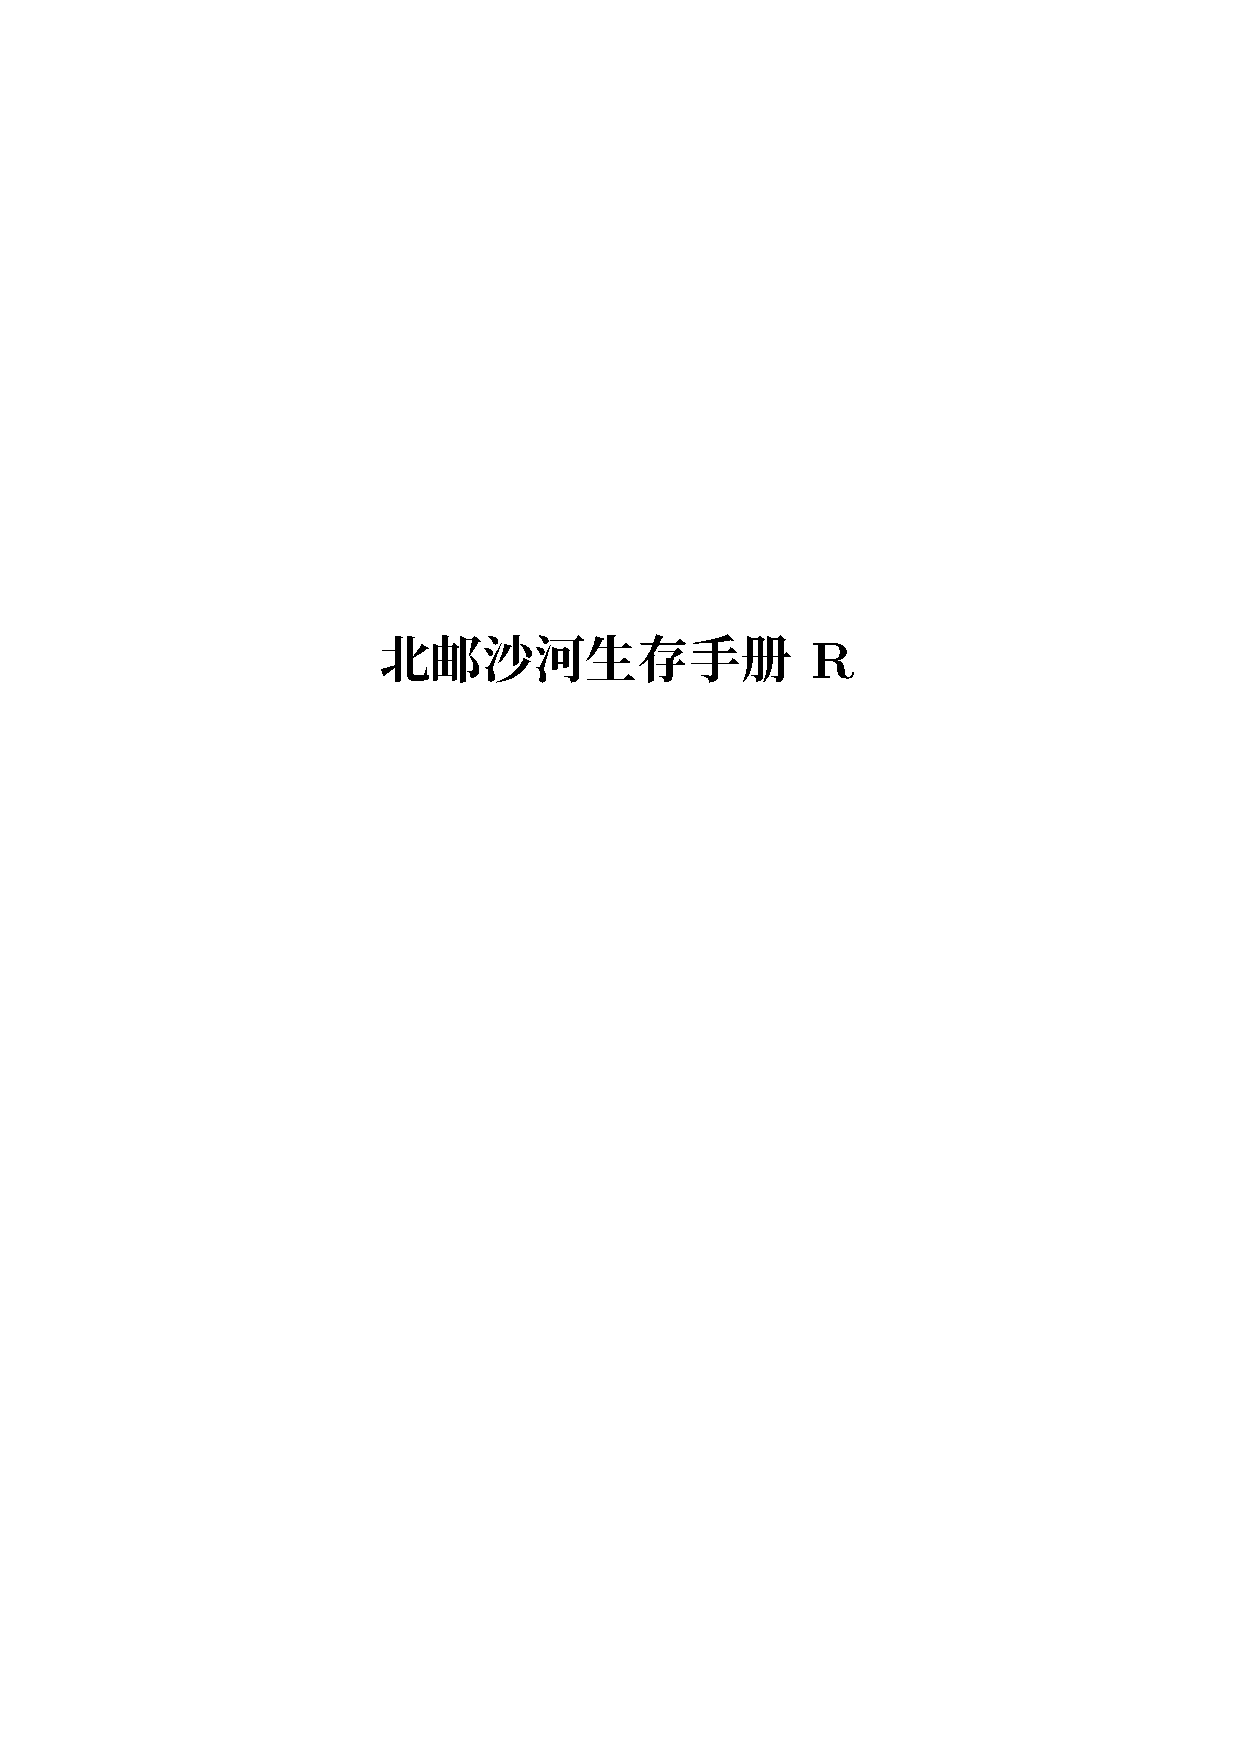
\includepdf{cover.pdf}

\begin{titlepage}
    \centering
    \vspace*{\stretch{1}}
    {\Huge\rmfamily\bfseries 北邮沙河生存手册R} \\[6.5ex]
    {\Large\sffamily 北邮软件工程根据地\ 群} \\
    \vspace{\stretch{3}}
    {\large\sffamily v2.0.1, July 2022}\\[1.5ex]
    \vspace{\stretch{0.5}}
\end{titlepage}

\begin{titlepage}
    \centering
    \section*{声明}

    本作品由“北邮软件工程根据地\ 群”的群友集体创作。\\
    可以在\href{https://github.com/BUPTSE/welcome}{此}获取本文档的源代码。

    \smallskip

    本内容以“CC BY-SA 4.0”许可证共享。要查看该许可证,可访问\\
    \href{https://creativecommons.org/licenses/by-sa/4.0/}{https://creativecommons.org/licenses/by-sa/4.0/}

    \smallskip

    受相关政策变化影响,部分内容可能有失准确,请以学校方面要求为准。

    \bigskip
    \tableofcontents
\end{titlepage}

\pagestyle{fancy}
\lhead{\small \leftmark}
\chead{}
\rhead{\small 北邮沙河生存手册R}
\lfoot{}
\cfoot{\thepage}
\rfoot{}
\renewcommand{\headrulewidth}{0.4pt}
% \renewcommand{\footrulewidth}{0.4pt}


% 新生报到
\section{新生报道}

\subsection*{学号与班号}

首先欢迎2022级软件工程的同学们加入这个豪华\sout{孤儿院}大家庭!
当你正式来到北邮的时候,便会得到两串十位数字:学号和班号。我们依次解读:
\begin{itemize}
    \kaishu
    \item 学号:2022(年份)21(全日制本科生)XXXX(四位学生编号)
    \item 班号:202121(同上)13(计算机学院\footnote{计算机学院(国家示范性软件学院)})16/17/18/19/20(软件工程的五个班\footnote{按照2021年的分班方法,这五个班以及一个双培班会成为四大班})
\end{itemize}

接触许许多多的新账号时不必头疼,优先尝试账号为学号,密码为身份证后6/8位或者8位生日的组合,能解决80\%的问题。(注意,身份证号含有X的需要大写)

\subsection*{报到流程}

% {\heiti 【待修改】开学时间节点(2021年)}
% \begin{itemize}
%     \kaishu
%     \item 8月27日 报道
%     \item 8月29日 9:30-11:00 2021级本科生英语入学分级及免修资格考试
%     \item 8月30日-9月12日 沙河校区校内军训
%     \item 9月13日 正式第一天授课
% \end{itemize}

报到的具体流程,在学校发放的新生手册中有详细介绍。通常来讲,大概分为宿舍入住、报到登记和一卡通办理、入校核酸等部分。这几部分一般没有顺序要求,强烈建议首先完成宿舍入住手续的办理,把行李丢在宿舍以后再去办其他手续会方便不少。

报到当天会有志愿者在北京站、北京南站、北京西站给坐火车的同学们接站,到学校以后也会有志愿者(就是学长们啦)全程接驾,千万不要紧张哦~

\newpage

% 校区环境
\section{校区环境}

北邮现在使用中的校区一共两个,即西土城路校区(海淀区,本部)和沙河校区(昌平区)。\footnote{另有西城区小西天校区(校舍)和昌平区宏福校区(接近弃用),目前和大家关系不大}校本部位于海淀区西土城路10号,面积很小,住宿条件相对较差,但交通便利,对面就是北师大,周围没事众多。目前,大三大四的本科生及多数研究生在本部学习。沙河校区是新生入学的校区,位于昌平区沙河镇南丰路{\small{}与高教园南三街交口向北400米路东\sout{(我知道写这些你不会看的)}}。规划面积很大(大概本部三倍)但是实际建成只有一半左右,住宿学习环境好,但比较偏僻,被两个地铁站夹在中间导致出行不便。沙河校区主要容纳大一大二学生。

按照学校最新的安排,计算机学院包括软工在内的学生都将只在沙河待一年,大二的时候就会搬到本部,所以今年沙河就只有22级的新生啦。

\begin{center}
    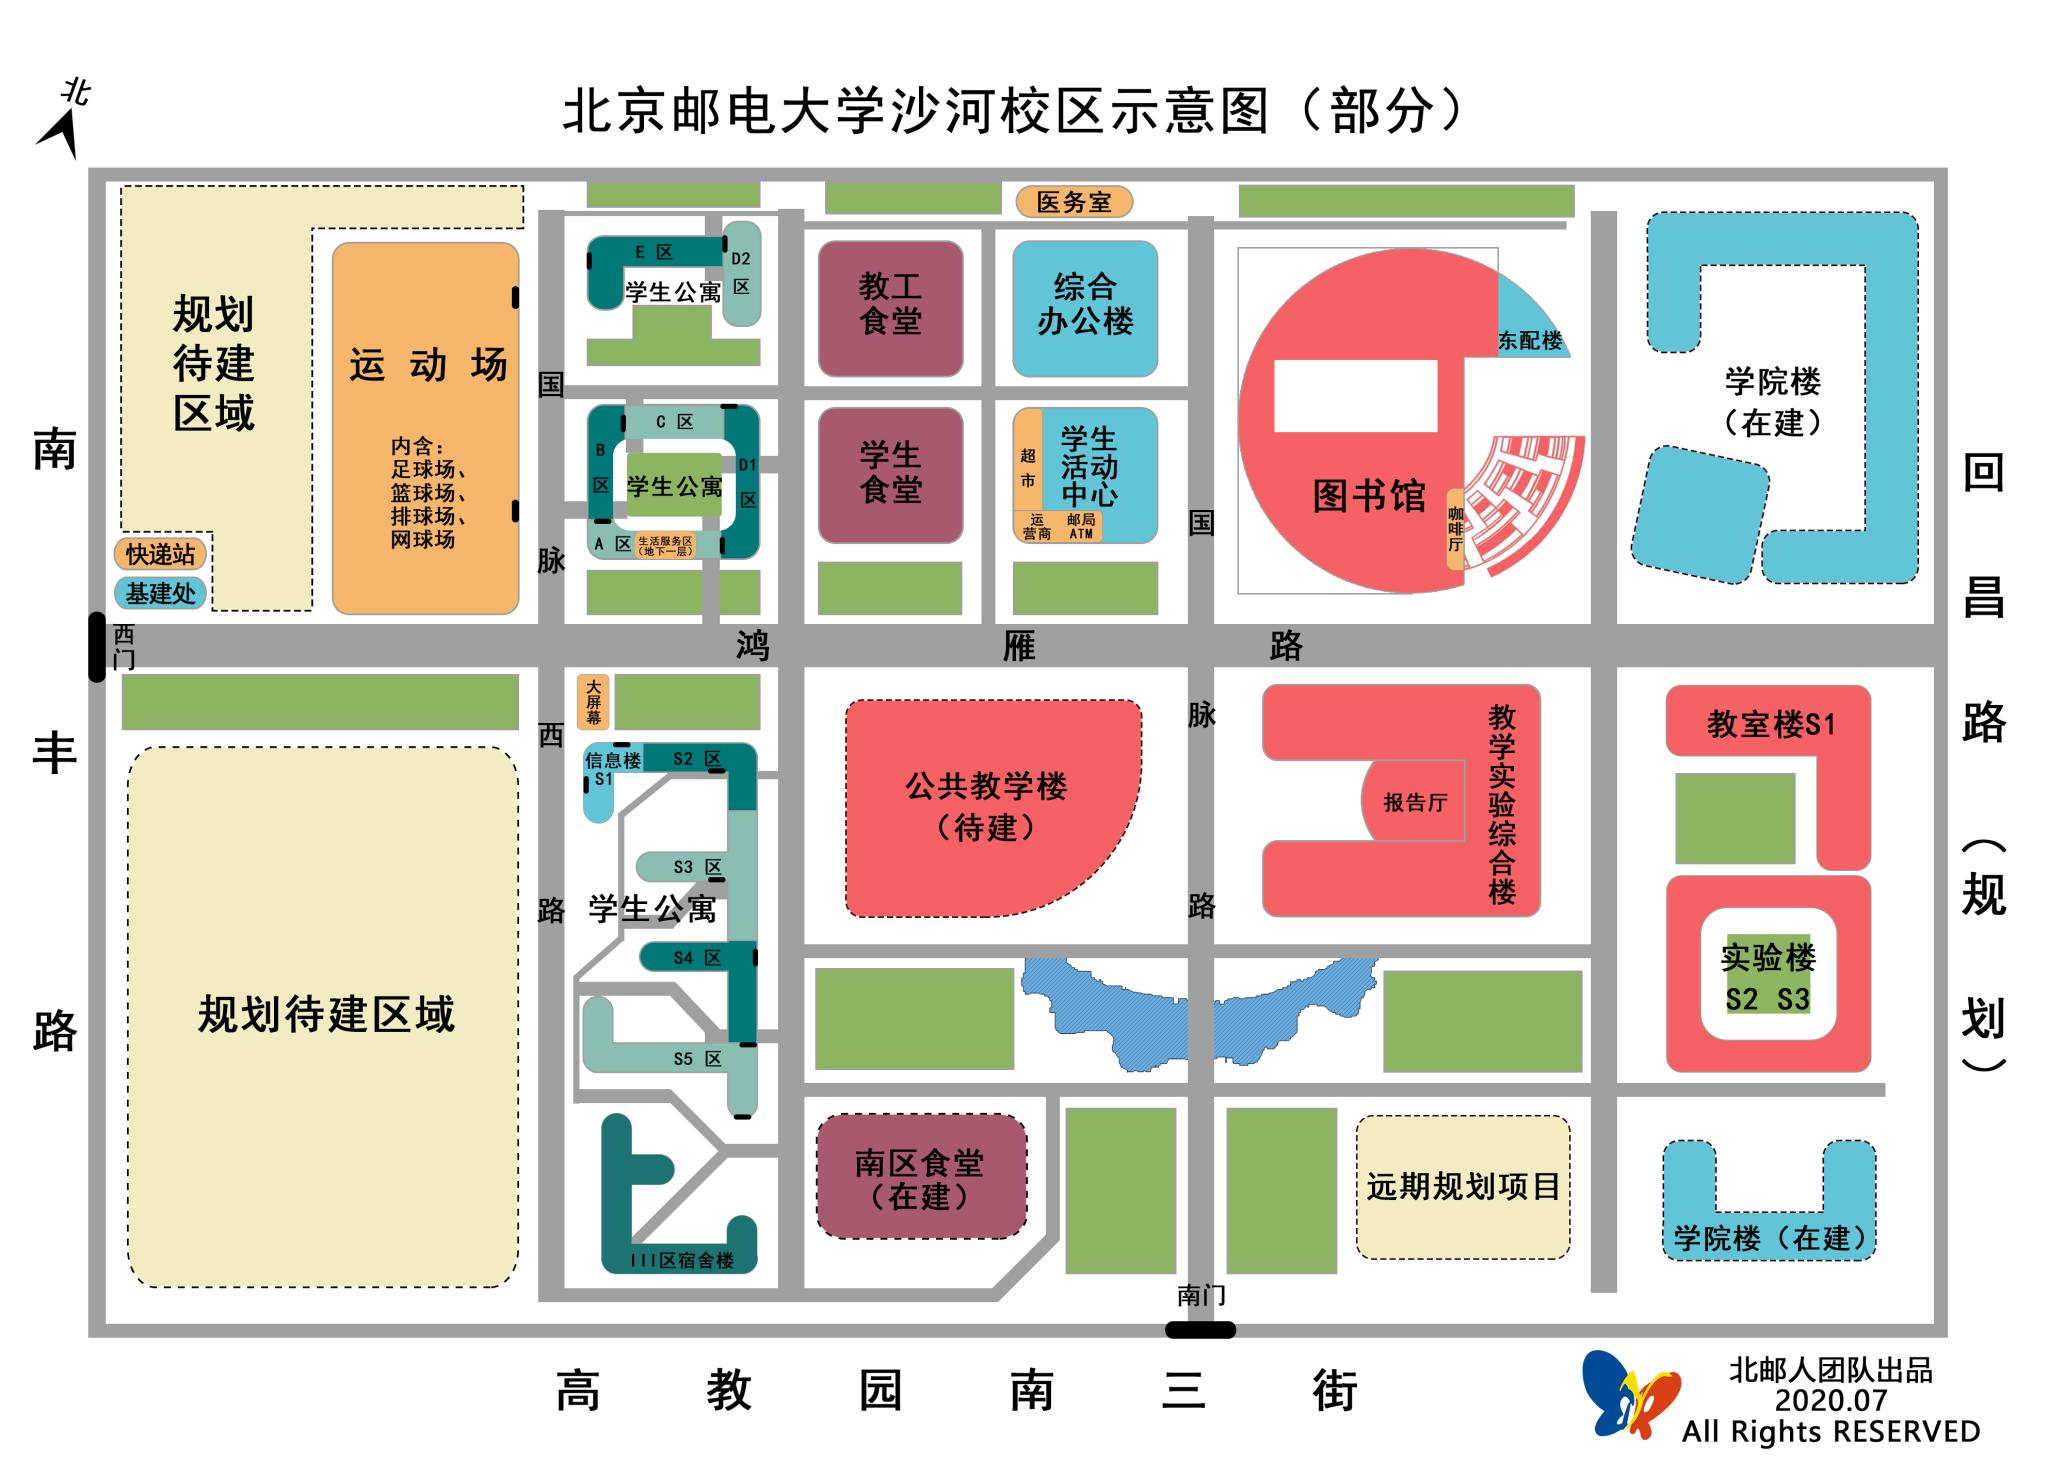
\includegraphics[width=0.80\textwidth]{images/shahe-map.png}
\end{center}

\faq{校园到底有多大?绕一圈要多久?}

很小,真的很小。本部绕一圈仅需10分钟,沙河大概也就20分钟(由于四周还没建设完成,所以(从物理上)根本无法绕圈(笑))。{\small (不过小也有小的好处,比如说可以7:55起床去上8:00的课)}

\faq{我什么时候会从沙河搬到本部?}

学校已经在招生章程中修改了各专业的办学地点。从2022级本科生开始,大部分学院(包括计算机学院在内)的大一会在沙河校区完成,大二至大四均会在校本部就读。\footnote{可在\href{https://zsb.bupt.edu.cn/info/1005/1720.htm}{此}查看各专业办学地点}

\faq{学校现在疫情管控严吗?能不能出去玩啊?}

根据学校目前的政策,出入校采取备案制(但疫情严重时会改为审批制,需要导员同意),不隔夜的情况下自动审批,大家白天出校门应该是没问题啦!关于疫情防控,现在学校内主要措施是进出建筑要戴口罩、测体温和扫二维码,部分食堂的桌子上有隔板,建议大家错位就餐哦(当然也不强制)。上课、体育锻炼和取快递外卖不受影响。

当然,入学后一定会有每日填报信息,大家不要忘哦。虽然也有自动打卡脚本,不过目前严抓,大家还是动动小手自己打卡吧(

\faq{有校车吗?免费吗?}

有,校车往返本部和沙河,但只在工作日安排。学期开始后可以在学校公众号上查询具体班次。由于校车要优先服务老师和本部学生,所以有可能会没有位子。有部分时段的校车需要提前在公众号上预约。

理论上车费5元,比地铁便宜,现在由于刷卡机故障,无需付费。正常情况下需用时35-55分钟,相较于地铁会更快一点,不过昌平线南延段修好以后就不一定了。

\faq{寒暑假我可以住在学校吗?}

目前由于学校规划调整,两个校区寒暑假都不再封校,但受疫情影响可能难以通过假期留校审批。另需支付住宿费。(以届时通知为准)

\newpage

% 住宿条件
\section{住宿条件}

\subsection{沙河宿舍简介}

根据宿舍楼的位置,沙河校区的宿舍分为雁北园和雁南园。相对而言,雁北园的条件会差一些,比如阳台空间较小、公共浴室较为破旧和储物空间较少。但其实也只是差一点(

\emph{雁北园}位于鸿雁路北侧,A/B/C/D1是四栋矩形相连的宿舍楼(一楼入口独立,二楼以上的部分相连),D2/E是另两栋独立于A/B/C/D1宿舍楼且相对较小的宿舍楼,内部也是相连的。离食堂操场生活区较近。雁北园各区域的代号为A/B/C/D1/D2/E。

\emph{雁南园}位于鸿雁路南侧,S2 S3 S4 S5是四栋平行的宿舍楼,六层,离教学楼和景观湖(线程池?)较近。南区食堂也修好了,即将投入使用。S6是一栋单独的宿舍楼,由于2020年才投入使用,所以条件是全校最好的。雁南园各区域的代号为S2/S3/S4/S5/S6(S1是信息中心楼)。

学校有三栋教学用楼宇的名字也是S1(教学楼)、S2(学院楼)和S3(实验楼),不要和宿舍楼弄混哦。S2 S3 S4 为男生宿舍,互通;S5 S6为女生宿舍(实际有三个不相通的部分)。按照学校的安排,所有的女生应该会统一入住S4,S5和S6,其中S4为男女混住,其余宿舍均为男生宿舍。

\subsection{宿舍环境}

无论是雁北园还是雁南园,宿舍的基本配置都是:四人间,上床下桌,有独立卫生间。卫生间内只有一个坑位和洗脸面盆,不能洗澡(但有地漏)。有的宿舍楼的独立卫生间会分成两个部分,分别是坑位和洗脸池。厕所里没有垃圾桶,需要自己购买。房间内有空调和暖气片,有阳台。

\begin{center}
    \begin{minipage}{0.45\textwidth}
        \centerline{\sffamily\small 雁北和除S6以外的雁南宿舍}
        \centerline{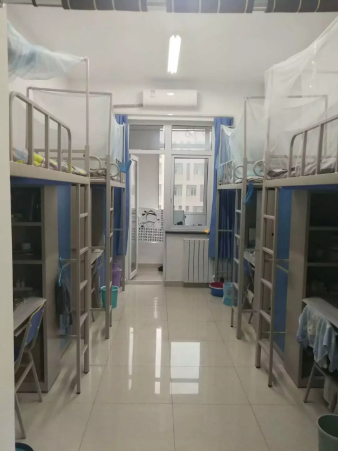
\includegraphics[width=1\textwidth]{images/dorm.png}}
    \end{minipage}
    \qquad
    \begin{minipage}{0.45\textwidth}
        \centerline{\sffamily\small 雁南S6宿舍}
        \centerline{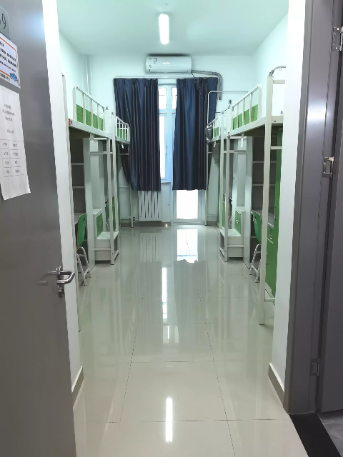
\includegraphics[width=1\textwidth]{images/dorm-s6.png}}
    \end{minipage}
\end{center}

\faq{我需要带什么生活用品吗?}

其实你可以什么也不带,报道当天都可以去学校超市购买。当然你自己带好常用的洗漱用品、床单被套啥的也可以。(非必须物品建议提前物流、网购或现场买,不建议千里迢迢携带)

\faq{宿舍楼还有其他配置吗?}

每层楼有一个公共卫生间和澡堂(如果不想经常清理房间里的厕所,建议多去公共卫生间),一楼有宿管的值班室,可以使用微波炉。每栋楼有一个电梯,一楼有若干自动售货机(买饮料零食泡面啥的),支持移动支付。部分楼层会有空出的房间作为自习室。

\faq{澡堂是怎么样的?}

纯淋浴房。采用刷卡计费的方式,大概每分钟0.1元。澡堂中午12:00到晚上23:00开放(其实管的不严的情况下一般不锁门),建议最好还是提前去洗,晚上的时候人还是比较多的。实测全天有热水,多放一会儿即可。雁北E区、雁南S6的澡堂拥有隔板,其他澡堂暂无。

\faq{宿舍楼有门禁吗?}

没有,但有宵禁。宿舍楼开放时间是早上6点到晚上11:00,如果要十一点以后回宿舍,就要提前联系辅导员进楼。带外来人员进楼要在宿管处登记。

\faq{水电费怎么算?}

水费目前没有收。电费每人每学期赠送40度电(所以宿舍四个人一共赠送160度)。电费价格:12元可购买25度电(只有空调最花钱,要不然花不了多少电)

\faq{上床下桌的尺寸是多大?}

\begin{center}
    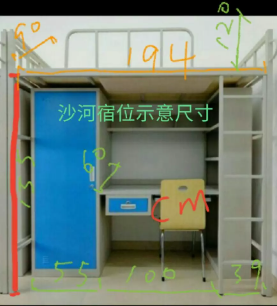
\includegraphics[width=0.55\textwidth]{images/bed-size.png}
\end{center}

又到了搬出老图的时候——不同宿舍的柜子尺寸可能不同,上床离天花板大概一米多一点,桌子上可以放得下27"显示屏。

\faq{我太高了,床不够长怎么办?}

报到前可以提前申请更换加长床,同时购买加长的床垫(要求190cm以上)。

\subsection{宿舍生活}

\faq{我会和我的同班同学住一个寝室吗?}

一般会,但也可能和同专业的其他班同学住一起。极端情况下你会与其他专业的同学一个寝室。分寝室结果在报道前可以在\href{https://welcome.bupt.edu.cn/}{迎新系统}上查到。\footnote{宿舍通常由辅导员分配,开学前辅导员应该会把你拉进一个QQ通知群,如果有特殊需求可以单独沟通}

\faq{辅导员会检查宿舍吗?}

开学后会有宿舍评比,主要看装饰和整洁度,可能会影响德育分(关于德育分的问题详见后文),具体看学院政策。辅导员查寝的频率取决于你的导员有多懒,以及学院有没有发动什么相关运动。

每周会有宿管卫生检查(实际上没来过几次),按百分制进行计分,基准分为100,不符合规定的倒扣对应分数。

\faq{宿舍装饰有什么限制吗,可以拉床帘吗?}

规定上不允许安装床帘,实际执行上不严。有部分宿管会限制蚊帐、床帘和地垫,可以尝试和他们理论,无果的话就不要装啦,具体购买之前可以先询问宿管和辅导员。不可以使用大功率电器(具体限制可以参看贴在宿舍门上的须知)

\faq{宿舍限电吗?晚上是否拉闸?}
沙河校区的宿舍都比较新,因此没有严格限制宿舍用电功率。规定上不得使用大功率电器和电热器具,实际上也并不会因此跳闸。晚上不拉闸,二十四小时通电通网。

\newpage

% 学业相关
\section{学业相关}

\faq{有开学考试吗?}

有且仅有一门:本科生英语入学分级及免修资格考试。难度高于高考(以全国卷为标准),大概略难于四级。听力部分与四级一样在卷面上没有问题,许多同学可能不适应。

分级考试的前1000名可以在大一上学期(12月)即参加四级考试,其他同学至少在大一下才能考四级(以学校通知为准);前120名左右可以申请免修综合英语4,之后还要再通过免修考试才能免修(关于免修问题下文将详细解释)。按照有关规定,批准免修的人数不超过60人,19级实际成功30人,20级由于疫情原因没有这个考试,21级实际成功30人。

除此以外,本次考试将会作为英语能力分级的依据。不同等级将会在大一、大二学年体验到不同难度的英语课程。计算机学院(国家示范性软件学院)英语课程模式为“2+2+2+2”,即在大一上到大二下的四个学期内,每个学期均有2学分的英语课程(每周上2课时)。课程设置情况如下:

% 最后没有把垂直对齐改成居中对齐,是因为长表格可能有跨页
\begin{center}
    \begin{longtblr}[
        caption = 英语课程设置情况
    ]{
        colspec = cclcc,
        hlines,
        vlines,
    }
        层次 & 学期 & \SetCell{c} 课程名称 & 学分 & 周学时 \\
        \SetCell[r=8]{h} 基础 & \SetCell[r=4]{h} {第一学期 \\ 必修} & A 级:综合英语 4 & 2 & 2 \\
        & & B 级:综合英语 3 & 2 & 2 \\
        & & C 级:综合英语 2 & 2 & 2 \\
        & & D 级:综合英语 1 & 2 & 2 \\
        & \SetCell[r=4]{h} {第二学期 \\ 必修} & A 级:公众英语表达与沟通 & 2 & 2 \\
        & & B 级:综合英语 4 & 2 & 2 \\
        & & C 级:综合英语 3 & 2 & 2 \\
        & & D 级:综合英语 2 & 2 & 2 \\
        \SetCell[r=6]{h} {提高/发展 \\ 目标} & \SetCell[r=3]{h} {第三学期 \\ 必修} & A 级:学术英语入门 & 2 & 2 \\
        & & B/C 级:英语听说 2 & 2 & 2 \\
        & & D 级:综合英语 3 & 2 & 2 \\
        & \SetCell[r=3]{h} {第四学期 \\ 限定选修} & {A 级:下列课程八选一 \\(不含公众英语表达与沟通、\\学术英语入门)} & 2 & 2 \\
        % 下面这行多少沾点摆烂了,,实在不知道该怎么搞
        & & {B/C 级:下列课程十选一 \\ ★ABC级打通排课 \\ \quad ●专门用途英语类:\\ \quad ①科技英语阅读与翻译 \\ \quad ②商务英语与国际交流 \\ \quad ③学术英语入门 \\ \quad ④实用英汉翻译 \\ \quad ⑤思辨阅读与写作 \\ \quad ●跨文化交际类:\\ \quad ⑥跨文化交际英语 \\ \quad ⑦情景英语视听说 \\ \quad ⑧英美影视英语 \\ \quad ⑨英美文化概况 \\ \quad ⑩公众英语表达与沟通} & 2 & 2 \\
        & & D 级:综合英语 4 & 2 & 2 \\
    \end{longtblr}
\end{center}

\faq{我可以不购买教材吗?}

可以,教材购买是自愿的。你可以不买教材或者从学长学姐手中购买二手教材。学期初的统一征订将会享有一定的折扣(定价的88\%左右),可以按需订购。学期过程中很可能不能再从学校教材中心补买教材,不过可以选择网购。许多地方都可以找到电子版的教材,如果遇到不能到校上课需要远程教学的情况,老师一般也会提供电子教材。

\faq{我的成绩怎么计算?}

成绩主要分为两类,每学年评定的综合素质评价成绩(主要用于排名并发放每学年的奖学金)和在第6学期结束后评定的专业综合成绩(用于确定推荐免试攻读研究生(俗称保研)的名单)。

根据\href{http://my.bupt.edu.cn/content.jsp?urltype=news.NewsContentUrl&wbtreeid=1025&wbnewsid=95500}{北京邮电大学本科生综合素质评价办法(试行)(校发〔2021〕52号)}的相关规定,自2021级起:
\begin{center}
    \emph{学年综合素质评价成绩\\=基本素质成绩×10\%+专业素质成绩×70\%+发展素质成绩×20\%}
\end{center}

基本素质成绩=班级评议成绩-扣分项。班级评议成绩满分为100分,包括政治思想(25分)、学习态度(25分)、道德品质(20分)、法纪观念(15分)、健康生活(15分)。扣分项主要参考违规违纪、全校通报批评等。

专业素质成绩为课程学分加权成绩,包括必修课(含体育课)和专业选修课程(按首次成绩计算),不含全校任选课、辅修课程。所谓加权成绩即所有涵盖的科目成绩按照学分权重计算平均分,免修英语不计入内。简单来说,学分越高的科目,权重越高。

发展素质成绩(俗称德育分)每学年通过年级制定的统一标准进行评定。无不良记录、参加志愿活动、实践活动和在学生组织担任职位有助于提高德育成绩。具体需依照当年的德育分评定细则,但大致组成框架如下:

\begin{center}
    \begin{longtblr}[
        caption = 德育分组成参考
    ]{
        colspec = {X[2, c] X[3, l] X[1, c] X[6, l]},
        hlines,
        vlines,
    }
        类别 & \SetCell{c} 项目 & 占比 & \SetCell{c} 主要内容 \\
        \SetCell[r=3]{h} 身心健康成绩 & 体能测试成绩 & 20\% & 体质健康测试 \\
        & 体育锻炼成绩(健步跑) & 10\% & 在运动世界校园中每学期的跑步公里数 \\
        & 身心健康活动评价成绩 & 10\% & 参与身心健康活动等 \\
        \SetCell[r=5]{h} 其他发展素质 & 思想成长 & 14\% & 参与主题教育活动,集体荣誉等 \\
        & 学术创新 & 14\% & 参与学术类活动及相关荣誉 \\
        & 美育素养 & 12\% & 参与美育类活动及相关荣誉 \\
        & 劳动素养 & 12\% & 社会实践,社团公益等劳动活动 \\
        & 组织协调能力 & 8\% & 党团班学(含学生社团)组织工作 \\
    \end{longtblr}
\end{center}

根据\href{http://my.bupt.edu.cn/content.jsp?urltype=news.NewsContentUrl&wbtreeid=1036&wbnewsid=95475}{北京邮电大学推荐优秀应届本科毕业生免试攻读研究生管理规定(校发〔2021〕50号)}的相关规定,自2020级起:
\begin{center}
    \emph{专业综合成绩=专业成绩(100分)+实践活动加分(上限4分)}
\end{center}

专业成绩的计算方式类似于奖学金中的“专业素质成绩”,即必修课、专业选修课的课程加权平均分,俗称智育成绩。

实践活动包括学术类竞赛、科研实践活动、体育类竞赛、文艺类实践活动以及退伍复学五个方面,成果及其对应加分,由学院根据北京邮电大学关于本科学生参加各类实践活动认定的实施细则(校发〔2021〕51号)的相关规定进行细化。

推荐免试攻读研究生(保研)除按照专业综合成绩排序外,还有一些基本条件:
\begin{itemize}
    \kaishu
    \item 前三年综合素质评价平均成绩须在其专业60\%(含)以内
    \item 前三年体质测试平均成绩须达到60分及以上
    \item 前三年完成劳动教育学时不低于24学时(该学时计算截止时间为每年8月31日)
\end{itemize}

\faq{什么是培养方案?我怎么看培养方案?}

培养方案是学校为每个专业制定的培养目标(最低毕业标准)。里面包括了你本科期间需要修读的课程,参与的实践活动和其他详细事项。培养方案会在开学后由辅导员发给大家,厚厚一本,也可以找辅导员要电子版。拿到培养方案后一定要仔细研读!

虽然很多地方都和你没太大关系,但也有很多需要注意的地方:首先你要对你每个学期所需要的学习的课程有一点了解,培养方案中有一张流程图,几乎是非常详尽的画出了每个学期的理论课和实习课。如果不出意外情况,课表就会根据培养方案来安排。重点关注一下学分比较高的课程,这些都是不能挂的重要科目。然后你可以找到任选课表和专业选修课表,提前规划一下你的选修课。此外还可以找到每个院的辅修安排,如果你大二以后想辅修一个专业,可以先看一看。(然而不建议辅修,建议专精一项)

\faq{什么是德育分?德育分怎么拿?}

德育分,或者说德育成绩,主要是指代学生除智育、体育素质外的其他综合素质。在2021级起的综合素质评价里主要表现为:基本素质成绩、身心健康活动、其他发展素质(这些名词的含义可见前文)。

基本素质评价几乎相持由平时的各项评价指标决定,包括青年大学习的完成率、打卡缺勤的次数、宿舍查寝的分数等,还有一部分是由班级同学匿名打分得来。(班级评议成绩=学生自评成绩×10\%+班级同学互评成绩×70\%+辅导员、班主任评议成绩×20\%)

而发展评价则“各凭本事”(论参加活动体现在何处)。因此要想德育分得分高,需要积极主动地参与各类活动(尤其是院内)(虽然不鼓励过于功利地参加活动,但活动之间确实存在有“认定”与“不认定”的情况,只能说本学院主办的活动具有天然优势)

德育分会在每学年秋季学期开始时评定(即大二的秋季学期评价大一学年的德育分,以此类推),奖学金的评定也是如此。(在口口相传过程中,经常会出现“德育分”和“综合素质评价成绩”不分的情况,比如上文)

\faq{奖学金怎么评?其他评优评奖呢?}

在秋季学期,综合素质评价成绩认定后,会开展一次本科生评优表彰工作。本科生评优表彰工作的基本条件是:无不及格课程成绩(必修课、专业选修课、体测)。

奖学金评定一般依照当年综合素质评价成绩依次选取(不重复),实际操作过程中一般会公示每个人获得什么奖学金,然后在学工系统中申请相关奖学金、荣誉称号。

\begin{center}
    \begin{longtblr}[
        caption = 奖学金与荣誉称号情况
    ]{
        colspec = {X[2, c] X[3, l] X[2, c] X[2, c]},
        hlines,
        vlines,
    }
        类别 & \SetCell{c} 奖项名称 & 名额 & 金额 \\
        \SetCell[r=6]{h} 奖学金 & 国家奖学金 & 1\% 左右 & 8000 \\
        & 学校一等奖学金 & 3\% & 5000 \\
        & 学校二等奖学金 & 10\% & 3000 \\
        & 学校三等奖学金 & 25\% & 1000 \\
        & 各类企业奖学金 & 以通知为准 & {8000/5000 \\ /3000/1000} \\
        & 国防奖学金 & 符合评选条件 & 按规定执行 \\
        \SetCell[r=2]{h} 奖学金(注册困难生专项) & 国家励志奖学金 & 依教育部下发名额而定 & 5000 \\
        & 企业奖学金 & 以通知为准 & 3000/1000 \\
        \SetCell[r=6]{h} 荣誉称号 & 三好学生 & 10\% & 500 \\
        & 优秀学生干部 & 5\% & 500 \\
        & 文体积极分子 & 5\% & 300 \\
        & 学习进步奖 & 3\% & 300 \\
        & 本科生先进班集体 & 20\% & 奖状一张 \\
        & 本科生优秀学生宿舍 & 10\% & 奖状一张 + 小奖品(生活用品等)
    \end{longtblr}
\end{center}

除了个人荣誉之外也有一些集体荣誉,如本科生优秀班集体和本科生优秀学生宿舍等。以上各类荣誉的评选方式届时会具体通知。

\faq{选修课怎么选?我该选什么课?}

每学期都会有任选课的机会,选修会在学期开始前在教务系统上\sout{抢}选课,选修课程表会提前放出,任选课主要可以分为:
\begin{itemize}
    \kaishu
    \item 理科类:数学物理有关的课程
    \item 工科类:各个院开设的专业相关选修课
    \item 艺术类:音乐美术电影相关的课程
    \item 人文社科类:政治、经济、历史、语言等相关课程
    \item 体育类:任选的体育课
\end{itemize}

除了体育类以外,本科期间剩下四类中与你所学专业无关的类别每个人都必须至少修读一门。以软件工程专业为例,则艺术类与人文社科类各需要至少修读一门。具体要求请参考你的培养方案。这个政策每年也可能会改变。如果你已经修满了所需学分,就可以不再选修任选课。

以上课程中部分是在智慧树等网课平台上课,这类网课名额多,没有抢课压力,不用按时上课,刷视频线上答题就能过,但内容比较水,是刷学分利器。由于疫情,大部分其他课程也都改成了线上授课,一般都是在腾讯会议等平台直播授课。这些(本应线下授课,但由于疫情改成线上授课的)线下课有的要期末考试,有的期末只要完成相应考核任务(写小论文之类)就可以给分。

选择任选课先以修满学分为目标,每个类别里面选一些你有兴趣的,然后可以咨询一下学长学姐课程的质量如何,考试难易程度如何,还要看看运气能不能抢到。你可以在一些地方看到总结好的公选课避雷指南,抄作业即可。选修课的具体开课列表常常变动,有的课每年作业量及给分也会有不小的变化,此部分经验进攻参考。抢不到课或者上课后发现不喜欢,在开任选课两周后有一次退补选机会。这里说几个热门的课程:

高等数学解题方法:仅大一开课,枯燥但最有用,每学期开两个班,基本爆满。考试前没有选的也去蹭课,但要考试。建议不选然后去蹭课。

公共日语、公共法语:同样爆满\sout{,但必须大二以后才能选},课时是其他选修课的两倍(也就是一周上两次),但学分也是两倍。

诺贝尔物理学奖史话:首次使用全息投影双校区同时授课的课程。

MATLAB应用:秒空课程之一,比其他几个语言啥的都快。

乐理基础:避坑课程,如果没有基础考试极易挂科(本条来自学长学姐告诫)

需要注意的是,任选课的成绩是不计入综合排名和保研排名的,但会出现在申请国外高校时需要使用的成绩单上,影响你的GPA。如果成绩实在不理想可以干脆挂科,只要后续不再选修这一门任选课,挂科记录就不会出现在成绩单上。

除了任选课以外还有专业选修课和英语、体育选修课(大二开始才有),具体参考你的培养方案。这些选修课都必须修满对应学分,基本上是二选一三选一系列,记得千万不要忘了选。

\faq{课表的时间安排是怎么样的?}

上午最早课程是8:00,最后一节12:15下课(1到5节)

下午最早课程13:00,最后一节18:10下课 (6到11节)

晚上课程最早18:30开始,最晚20:55下课(晚课都是任选课,且实际上一般从19:20开始上课,不用担心没时间吃晚饭)

中午休息时间较短,如果碰到五六节联排会很难受。但这样为大家争取到了更长的假期……(目前看来2021级软件工程只有19-20班的星期四有这种困扰)

周三下午全校无课,时间可以用来进行各种实践活动(开各种会)

原则上周末不上课。

\faq{上课的安排是怎样的?}

大班课:如数学课、物理课等公共课,一般以大班为单位,一百多人在一个大教室里上课。

小班课:一般是专业课,一两个班级在一个小教室里上课。2020级是16-18班一起,19-20班一起。也有部分课程16-17班一起上课,18-19班一起上课,20班单独一个老师。对于21级而言,由于双培生单独成班,所以一般是16-18班一起上课,19-20+双培生的班级一起上课。

特殊的课程:英语课分级以后单独编班,一个班30人一起上课,听说课则是一个班在听力机房上课;各种上机实验课也都在机房上课(但一般你还是带自己的笔记本,最好不要指望用学校的电脑),还有一些课程在特殊的实验室上课。

\faq{作业写在哪里?怎么交?}

一般来说,作业有这么几种:

课堂派等线上平台布置的小作业:根据老师要求可以写在纸上拍照上传,有时也可以提交电子文档,ddl(截止日期)由老师设定,超时就算作缺作业(不过老师们一般都比较仁慈,补交也不是不行)

课前手动收的作业:一般写在纸上(也可以写电子版,具体看老师是否有明确要求),和你在初中高中写的作业差不多,由学委或老师指定的课代表统一收取。

上机作业:又称OJ作业,即线上编程测试,只有部分专业课有,这个到时你们就知道了。

大作业:一部分的课程会布置占成绩比重较高的大作业,有的个人完成,也有的以小组完成。这类作业会有详细的完成要求及提交说明,一般成品通过邮件提交。有的课程期中或期末并不考试,也以大作业形式完成考核。

哦对了,英语听说课则需要在专门的新理念平台上做线上答题作业,由于这个平台是在太拉胯了,你的电脑可能不会兼容,这时建议每两周抽一次没课的上午去上课的机房完成(当然有很多办法可以在寝室完成(甚至让脚本自动完成)该作业,具体的到时请咨询你身边的大佬)


\faq{每门课的最终成绩怎么算?翘课对成绩影响大吗?}

因课而异,一般是平时成绩+期中+期末,期末要占到40\%以上。

每个老师对平时成绩的定义不一,有的要求考勤+作业完成,有的只要求作业,有的甚至没有要求。但是尽量不要翘课,平时成绩好一点有助于你期末考试失利的时候老师拉你一把。

\faq{如何免修课程?免修的课程如何计算成绩?}

北邮现在不允许免修除了大一上学期的综合英语4以外的其他科目。要免修综合英语4,首先需要在入学时的分级考试中取得一个相当靠前的成绩,然后报名参加英语免修考试,经考核合格后即可获准免修此课程。免修的课程不计入最后计算的成绩,在成绩单上显示为“免修”。

以前也曾允许过免修其他课程,目前暂时没有恢复相关制度的消息。

\faq{从哪里可以获得学习资料以及历年的试卷?}

学习资料:获得途径有专业群、班级群、各个科目老师建立的课程群等等。你也可以从好朋友或者学长学姐那里取得一些秘藏资源。(在北邮人pt上有很多其他学校的好资源,关于pt站的介绍见“内网资源”一节)

历年试卷:由于\sout{懒得出题}众所周知的原因,往年的试卷通常是不会外传的(除了高等数学、线性代数等科目)。不过你可以询问你的学长学姐,他们有时会保留往年的试卷,也可以去打印店碰碰运气(一般打印店老板会保留每年同学们经常打印的资料)。或许还有别的一些奇怪的渠道能获得。

本群的群文件中有着非常丰富的学习资料,基本能涵盖你想要的所有,需要请自取。

\emph{需要注意的是北邮没有任何学生组织、大创项目、微信小组等“提供”或售卖高数、线代等热门课程的“内部”或“特供”资料,在QQ群和微信群等社交网络上宣传资料的陌生人均为社会组织或诈骗团伙,一定不要轻易上当!}

\faq{北邮的假期多吗?}

北邮江湖人称北京不调休大学,很多时候节假日都会连放很多天,即别人放假的时候我们放假,别人调休的时候我们还是放假。例如2022年的国庆,如果没有意外情况,大家可以享受到⑨天的超长假期。

\faq{我想转专业,应该怎么做?}

根据\href{http://my.bupt.edu.cn/content.jsp?urltype=news.NewsContentUrl&wbtreeid=1036&wbnewsid=25646}{北京邮电大学本科生校内转专业办法(校发〔2020〕14号)}的相关规定,符合条件的本科生可以在大一下学期初和大二上学期初提出转专业申请。转专业考核仅由接受转入学生的学院进行,各学院要求不同。一般由已取得的课程成绩和可能的笔试、机试成绩按比例计算出综合成绩,排名靠前的经面试后就可以成功转专业了。对于软件工程专业来说,想要转出的同学会比较少,更详细的信息可以咨询群里的学长学姐。

\newpage

% 生活相关
\section{生活相关}

\subsection{生活服务}

\faq{学校内有哪些生活服务?}

生活服务区在雁北园负一楼,有超市、文具礼品店、理发店、水果店、眼镜店和电子产品修理店,部分店价钱小贵但可以接受,支持刷学生卡或移动支付。

提示:如果是重度水果患者,可以考虑点外卖购买水果,可能比在水果店购买水果便宜。\sout{由于疫情封校,水果店老板跑路了,学校依据情况由后勤部门安排水果供应。}又来了个新的水果店老板

文具店的价格比较公道了,没必要另寻他路。超市里不定期会有打折商品和捆绑销售的商品,如果你能接受,那就是赚到。理发店价格20元一次普通理发,也可以染发什么的。如果觉得不好,可以去沙河镇上的理发店。(虽然我没去过(但是理发店的水平真是一言难尽(不过要是疫情封校也就只能接受了

学生食堂对面有一家名为小麦铺的商店,商品较为齐全,里面还有一家打印店和一家水果店。在打印店打印时要注意资料安全,有需要保密的资料请慎重。生活服务区的超市里也开了一个自助打印店,图书馆一层也有自助打印机,各种二手群里也可以寻到不少同学提供价格优惠的打印服务。

学生活动中心一层内有邮政门面和运营商的营业厅,以及另一家电脑修理店。此类修理店价格都比较贵,如果你的电脑只是需要清灰或者加装硬盘可以找身边的电脑爱好者搞定,二手群里也有同学以相当低的价格提供类似服务,如果电脑硬件出现比较大的问题,建议联系原厂售后。

在各种新生群以及校园内你可能会遇到推销手机校园卡套餐的人,如果你确实需要的话,可以在各个群里多方打听一下,寻找一个价格相对较低的售卡代理。

\faq{校内有洗衣房吗?}

雁北和雁南均有洗衣房,自助洗衣,5元一次,可以多加几元选择热水洗。你也可以选择在卫生间洗手池那里手洗。但是不允许自己购买洗衣机(因为用电安全)。

\faq{收发快递方便吗?}

根据快递公司不同,你会遇到下面几种情况:

中国邮政:学校亲儿子,门面设在学生活动中心一楼,收发快件都很方便,很便宜,但是比较慢(也就慢1-2天),但是营业时间有限(9:00-16:00)。

其他快递:学校门口的菜鸟驿站,分为手动取件和自动快递柜两个区域,自动取件柜怎么操作不用说了,24小时开启。手动取件要自己根据取件码找到快递+使用身份码出库,晚上七点关门,记得及时去取。

受疫情及校园管理影响,部分快递公司可能不能把快件送进校园,或者是封校时所有快递卡车均不能进校。因此,有可能出现京东、顺丰等等的包裹跟邮政的快件一块送到邮政门面,以及需要从围墙上方丢过来的或者干脆要到校门外去取的各种奇妙状况,需要多加注意。建议取快递前向消息灵通的同学打听一下。

\subsection{餐饮美食}

\faq{沙河有几个食堂?伙食怎么样?}

加上新建的南区食堂,一共有三个。已有的两个食堂在北侧二维码广场,分别俗称为学生食堂和教工食堂,各有五层,不论学生老师都可以用餐(不要被教工食堂这个名字给骗了,学生也可以去哦)\footnote{沙河的食堂命名比较混乱且经常变动,恐怕今后很长一段时间内都还会沿用“教”“学”“南”的俗称\\\hspace*{4em}学生食堂:地图中标示为风味餐厅,A 楼\\\hspace*{4em}教工食堂:地图中标示为教工餐厅,D 楼\\\hspace*{4em}南区食堂:地图中标示为学生餐厅,南区食堂楼}。除了教工食堂五层是点菜制的有包厢的餐厅(也是唯一可以使用移动支付和现金的餐厅),其他楼层都是窗口制。南区食堂由于刚刚投入使用,目前只工供应基本伙。

每天的窗口快餐菜单可以关注餐厅公众号(沙邮餐饮)查询。

基本伙:学三 教二 教三

美味快餐:学一 学二 教一

美食城:学四 学五 教四 教五

注:学/教+数字代表学生食堂/教工食堂的第几层

此外还有一家咖啡厅位于图书馆一楼东侧(环境非常舒适,服务到位,不过价格有点小贵);以及一个面包房(面包好硬,难吃)和一个西餐厅(实际卖汉堡薯条),位于学一食堂旁边。教学楼、学生活动中心、东配楼等都有自助咖啡机和自动售货机。

\faq{点外卖方便吗?}

学校在小南门\footnote{从西门进校后路的右侧(南侧)有一个小门,以前是一个栅栏铁门,现在拆除铁门改为了外卖柜}安装了外卖柜,学生点的外卖需要统一到外卖柜去取,从宿舍走个来回大约需要10分钟。

\faq{饮水方便吗?}

教学楼、图书馆、宿舍等楼层里面都有热水机,插学生卡即可使用,非常方便。寝室都可以不用热水瓶。也有一个水站提供桶装水,不过不是很有必要。

\faq{有哪些一般人不知道的美食?}

水果店里的糖葫芦:5块钱一根还贼好吃(15块钱的草莓糖葫芦也非常美味),数量有限记得每天下午早点去蹲点。

教四烤鸭架:虽然没有标出来,但你可以不花\sout{16.8}17.8买烤鸭套餐而选择6块一份的鸭架骨,分量大骨头上的肉也很多,物超所值。

\subsection{活动场所}

\faq{图书馆的开放时间?借阅规则?}

图书馆服务区早上八点到晚上十点开放(节假日另行通知),刷学生卡进入,一次可以借阅两本书,时长30天,可续借两次(每次可续15天)。一切操作都在自动借还机上完成(放假时自动续借)。如果超时归还,会遭到一段时间不能借书的惩罚,时间过长还会被罚款。

图书馆一共五层,每层均有很多自习座位,一层为自习区,不受放假闭馆时的限制,7:00-22:50开放,学习环境超级棒,建议需要认真学习时都来图书馆。

图书馆二楼提供查询资料的临时电脑,免费。此外还有自助打印机,不过价格比打印店要贵。

图书馆五楼有个小型博物馆,里面有远古电脑等有趣的展品。目前受疫情影响撤展了,恢复时间不明。

\faq{如果要小组讨论问题或者做大作业(或者和好基友闲聊),有哪些地方去?}

研讨间(推荐):图书馆的2-5楼均有,是环境很好的小隔间,可供2到8人进行研讨。需要在微信小程序上提前预约,预约的时候要选择使用时段(一次最多预约两个小时),并且必须有一人按时去打卡使用,否则会因为咕咕咕而受到惩罚(好像是三次违约后本学期不能预约)。因为房间有限,黄金时段很难抢到,建议必要的时候提前1天预约。环境较好,隔音能力中等(外面的人听不见,但是隔壁的人有可能听见)。部分研讨间设有大屏幕,可以连接电脑进行投影。如果需要大屏幕但你预约的研讨间里没有,你也可以和图书馆管理员协商一下,移过来一台。

教学楼教室:现在每栋教学楼的1楼都有智慧屏,可以查询教室的使用情况,找一个该教室没课的时候,大家都可以自由使用教室。大教室一般会有同学在里面自习,所以需要小组讨论,可以去N楼和S楼之间的小教室,教室周末也可以使用。S1教学楼的教室环境更好一些,有的还有移动白板可以使用,适合中等规模的研讨。如果需要举行会议或其他活动,可以通过学生组织或辅导员申请借用教室,在批准的借用时段可以独占整个教室。

塞纳左岸咖啡馆:在图书馆东侧一楼。环境很优雅,服务很周到,不过没有隔音,所以不要进行一些会很吵的活动,不过闲聊什么的倒是一个好去处。开放时间为早上9点到晚上10点。

学生活动中心:里面有很多各个部门专用的办公室、会议室,如果你加入了一些学生组织,可以联系当部长副部长的学长学姐,他们也许会“借”给你一个房间。因为不常有人来,所以环境非常安静,适合思考问题。

\subsection{交通往来}

\faq{我可以在学校里面滑滑板吗?}

可以!都可以!宿舍门口和教学楼门口用黄黑胶带划定了区域放置滑板,不过没有人看管,要小心失窃哦。

\faq{学校离地铁站太远怎么办?}

走(毕竟就1km)!或者骑自行车,自行车可以停在沙河高教园地铁站附近,上一个车锁基本可以保证安全(不要停在沙河站,那里人多眼杂)。

\faq{到底往南走坐地铁方便,还是往北走方便?}

往南沙河站,往北沙河高教园站,距离基本一致,但是往北走会导致你坐到三环左右就需要7元,从沙河站则只要6元。如果需要顺便购物,从沙河站下车附近有超市和餐厅。但是如果是高峰时段沙河站非常拥挤,提前一站坐车会舒服一点(别想了还是没有位子),并且相对人流涌动成分复杂的沙河站来说,沙河高教园站相对安全一些。

由于北京地铁昌平线采取大小交路运行,沙河高教园站会有始发车(空车!有座位!)。

\href{https://www.bjsubway.com/station/xltcx/linecp/2013-08-26/246.html?sk=1}{沙河高教园站列车时刻表}

\href{https://www.bjsubway.com/station/xltcx/linecp/2013-08-26/249.html?sk=1}{沙河站列车时刻表}

\newpage

% 军训相关
\section{军训相关}

\faq{军训时间与地点}

由于疫情原因,近几年的军训都在沙河校区校内举行(原本是在八达岭军训基地 )。

预计军训时间会从正常的大一上入学前推迟至大一下结束后的暑假。

\faq{军训内容}

\begin{itemize}
    \item 必修:齐步、踏步、正步
    \item 选修(随机分配):军体拳、擒敌拳、旗语等
    \item 活动:拉歌、看电影等
\end{itemize}

\faq{校内军训体验}

对于校内军训来说,除了军训期间的训练与活动外,其余与正常在校完全一致:你可以自由地洗澡、收快递、点外卖等,并没有任何差异。

这相比于在军训基地来说舒服得多(比如在军训基地14天只能体验3次限时铁链澡堂)。

想看往届军训基地的艰苦条件,可参考往年国防教育协会整理的军训生存指南。
\newpage

% 内网资源
\section{内网资源}

\newpage

% 学生组织
\section{学生组织}

\faq{沙河有哪些学生组织?怎么加入?}

粗略可分为校系、院系、社团系三个派系。

\emph{校系}:校团委、校学生会、社团联合会(现改为社团工作部,负责管理社团)、北邮青年新媒体中心、北邮鸿雁党媒、校运动队、真情志愿者联合会等

\emph{院系}:各个学院的团委、学生会、志愿者协会(计算机学院是星火志协)等

\emph{社团系}:即所有社团,还包括曾经是校系组织的大学生艺术团(2021年起改为社团)。在信息门户和群文件中有完整白名单,可仔细查阅。

加入校系学生组织要困难一点:团委、学生会、青梅、鸿雁、真情志愿者,他们都会在开学期间进行招新,需要进行一到两轮的面试才能加入,在高中有很强社会活动经验或者有一些技术上的特长会很有帮助。团委原则上要求必须是团员,如果你不是,也可以开学的时候和导员申请入团。

而加入院学生组织比较容易:院学生会也会统一组织招新,面试也比较简单,名额比较多。
如果这些面试你都挂了,还可以在班会的时候竞选班委,成功率也会很高。运动队大多是特长生招进来的,如果你不是专业的,就不要想了。

加入社团基本没有限制:一般而言如果你对某个社团感兴趣可以直接加他们的群,如果想要成为社团的正式成员需要在学校的学工系统中正式申请加入,每位同学最多可以正式加入两个社团。而中心组成员一般需要在10月通过报名、面试等环节进行筛选。(一般而言中心组成员才视为社团干事)如果你进入了某个社团的中心组,就相当于进入了该社团的管理层,需要负责安排对应社团的事物。如果只是普通正式成员,是不算校级学生组织的。

\faq{学生组织会很忙吗?都有哪些福利?}

最重要的:在德育分中有一定比重的职务分。(但是多个职务累加还是取最高就不一定了)
所以如果你想要更高的综测成绩,可以至少加入一个院/校级学生组织。

因为招新进入的同学都是干事身份,所以大多组织的活其实是不多的,基本是每个月或两个月组织活动的时候才会有分配任务。校/院级组织的活动频率低,但要求高,需要你花点心思完成你的工作。而班委基本只需要完成日常工作和导员的小任务,难度低但会比较繁琐。

学生组织和班委的任职年限都是一年,一年后就可以选择放弃职务或留下一年或竞选职务,如果竞选成功会升职为副部长之类的职位,可以获得更高的德育分评定,但也会更加忙碌。每个部在大二末期还会选择部长,除了部长一般大三以后不再担任学生组织的职位。因此如果你前两年不参加,后面就没有办法加入学生组织了。

不用担心学生组织会影响考试复习,考试周期间一般是不会安排任务的。但如果你遇到了很扯淡的老师/部门(点名批评社团工作部,考试周还给社团派活),那就不好说了。

各系学生组织都会有各种福利,包括但不限于:不定期聚餐(公费吃喝的很少,AA制的更多)、为你过生日会、组织各类娱乐活动,瓜分多余的活动奖品等等。并且你可以比其他同学更早获得学校活动的信息,有名额限制的活动(比如大学间联谊,观影会、公益演出等)可以获得内部机会不用抢票之类。并且你会有同部门的学长学姐可以指点迷津。一些大型活动的名额一般还是会更加青睐学生组织成员的。

\faq{如何参加大创活动?有哪些好处?}

在大一、大二年级可以参与雏雁计划(“大创的练兵场“)体验大创流程。一般为10月立项,次年4月结题。此后可以正式参与大创,一般于7月公布立项结果,次年6月进行评定。中间会有若干中期评定等环节,更为正式。

雏雁或大创获奖会在德育分评定上有加成,未来找实习简历上也可以多一些东西。

\faq{学校还有哪些经常举办的活动?}

学校的公共活动:运动会、电影公映会(《我和我的祖国》、革命者、五个扑水的少年)、进校园演出(19年看了开心麻花,疫情之后基本没有了)、各种类型的讲座等等。

社团活动:秋季学期游园会(百团大战),春季学期百花节,均为社团大摆摊的形式,玩得痛快。

每个院组织的大型活动:一般有歌手比赛(计算机学院的秋之韵)、表演比赛、辩论赛等。

大型志愿活动:比如2019年的国庆游行方阵,2021年的建党100周年庆祝大会,首都举行的各种会议,包括冬奥会,都会在大学生中招募志愿者。

\newpage

% 其他事项
\section{其他事项}

\faq{什么东配楼信息中心都是哪里啊,地图上根本找不到这两个地方啊?}

\emph{前文中的地图已经完整标注}

东配楼是在图书馆的东侧背后,是辅导员和一些老师的办公楼,根据图书馆楼下的指引可以找到。信息中心是雁南园靠鸿雁路路边的那一栋楼,代号为S1。和宿舍楼紧挨着因此经常被误认为是宿舍楼。里面是办理补办校园卡和学生账号等问题的地方。学校有一栋教学楼的名字也是S1,不要和信息中心弄混哦~

\faq{校园卡丢失了怎么办,可以补办吗?}

可以,去上文中的信息中心补办就可以了,需要交工本费,不过不限补办次数。里面的余额只要补办前不被盗刷,都可以保留。

\faq{学校办的银行卡是什么样的?有哪些补助?}

\begin{center}
    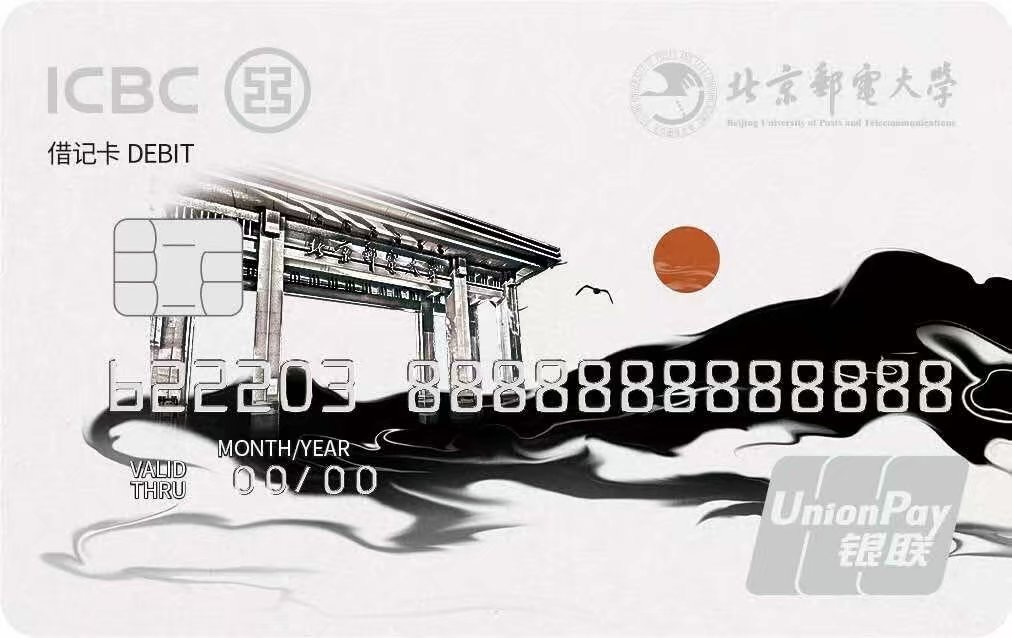
\includegraphics[width=0.55\textwidth]{images/card.jpg}
\end{center}

具体办理方法见录取通知书附带的新生指南。每人每月将获得北京市提供的60元生活补助(会发放到上述银行卡或校园一卡通中)。另有注册困难生的补助若干。

\faq{他们说的什么果园梨园树莓啊,都是什么东西啊?}

一些简称:
\begin{itemize}
    \item 果园:国际学院
    \item 梨园:理学院
    \item 树莓:数字媒体与艺术学院
    \item 青梅:北邮青年新媒体中心
\end{itemize}

课程简称:
\begin{itemize}
    \item 数电:数字系统基础
    \item 计组:计算机组织与结构(对于软件工程专业)
    \item 自动机:形式语言与自动机
    \item 大雾:基础物理学(对于软件工程专业)
    \item 软导:软件工程专业导论
    \item 思修,史纲,马原,毛概(也叫毛中特):四门\footnote{按教育部的要求,现在增加了《习近平中国特色社会主义概论》和“党史”“新中国史”“改革开放史”“社会主义发展史”四选一,共六门}思政课,按顺序一学期一门,分别为《思想道德基础与法律修养》、《中国近现代史纲要》、《马克思主义基本原理概论》、《毛泽东思想和中国特色社会主义理论体系概论》
\end{itemize}

\faq{我想参加某某竞赛/活动,如何报名/找到组织?}

对于以个人名义参加的竞赛或活动,一般来说等待学校发布相关通知后按要求报名即可。

对于需要组队参加的竞赛或活动,通常都需要一个指导老师并通过学校集体报名。程序设计竞赛由集训队负责组织,其他情况类似的竞赛一般也有现成的老师负责,你可以在各种群里询问学长学姐,相信很快就能找到组织。

如果你参加的比赛之前从未有人参加过,而又必须通过学校报名等等,你可以向学院和团委等有关部门询问相关事项。

\newpage


\includepdf{back.pdf}

\end{document}
